% % % % % % % % % % % % % % % % % % % % % % % % % % % % % % % % % % % % % % % % % % % %
%                                                                                     %
% Short Sectioned Assignment LaTeX Template Version 1.0 (5/5/12)                      %
% This template has been downloaded from: http://www.LaTeXTemplates.com               %
%                                                                                     %
% Original author:  Frits Wenneker (http://www.howtotex.com)                          %
%                                                                                     %
% Modified by: Fco Javier Sueza Rodríguez (fcosueza@disroot.org)                      %
%                                                                                     %
% Changes:                                                                            %
%	    - Custom Chapters, Sections and Subsections (titlesec package)                %
%           - Document type scrbook (oneside)                                         %
%           - Use babel-lang-spanish package and marvosym                             %
%           - Use hyperref, enumitem, tcolorbox and glossaries packages               %
%           - Use Time New Roman (mathptmx), Helvetic and Courier fonts               %
%                                                                                     %
% License: CC BY-NC-SA 3.0 (http://creativecommons.org/licenses/by-nc-sa/3.0/)        %
%                                                                                     %
% % % % % % % % % % % % % % % % % % % % % % % % % % % % % % % % % % % % % % % % % % % %

%-----------------------------------------------%
%	              Packages                  %
%-----------------------------------------------%

\documentclass[paper=a4, fontsize=11pt, oneside]{scrbook}

% ---- Text Input/Output ----- %

\usepackage[T1]{fontenc}
\usepackage[utf8]{inputenc}
\usepackage{mathptmx}
\usepackage[scaled=.92]{helvet}
\usepackage{courier}
\usepackage[indent=12pt]{parskip}

\usepackage{geometry}
\geometry{verbose,tmargin=3cm,bmargin=3cm,lmargin=2.6cm,rmargin=2.6cm}

% ---- Language ----- %

\usepackage[spanish]{babel}
\usepackage{marvosym}

% ---- Another packages ---- %

\usepackage{amsmath,amsfonts,amsthm}
\usepackage{graphics,graphicx}
\usepackage{titlesec}
\usepackage{fancyhdr}
\usepackage{tcolorbox}
\usepackage{hyperref}
\usepackage{enumitem}
\usepackage[automake]{glossaries}

%--------------------------------------------------------------------%
%                      Customizing Document                          %
%--------------------------------------------------------------------%


% ----------- Custom Chapters, Sections and Subsections -------------- %

\titleformat{\chapter}[display]
			{\bfseries\Huge}
			{Tema \ \thechapter} {0.5ex}
			{\vspace{1ex}\centering}

\titleformat{\section}[hang]
			{\bfseries\Large}
			{\thesection}{0.5em}{}

\titleformat{\subsection}[hang]
			{\bfseries\large}
			{\thesubsection}{0.5em}{}

\titleformat{\subsubsection}[hang]
			{\bfseries\large}
			{\thesubsubsection}{0.5em}{}

\hypersetup{
    colorlinks=true,
    linkcolor=black,
    urlcolor=magenta
}

% ------------------- Custom heaaders and footers ------------------- %

\pagestyle{fancyplain}

\fancyhead[]{}
\fancyfoot[L]{}
\fancyfoot[C]{}
\fancyfoot[R]{\thepage}

\renewcommand{\headrulewidth}{0pt} % Remove header underlines
\renewcommand{\footrulewidth}{0pt} % Remove footer underlines

\setlength{\headheight}{13.6pt} % Customize the height of the header

% --------- Numbering equations, figures and tables ----------------- %

\numberwithin{equation}{section} % Number equations within sections
\numberwithin{figure}{section} % Number figures within sections
\numberwithin{table}{section} % Number tables within sections

% ------------------------ New Commands ----------------------------- %

\newcommand{\horrule}[1]{\rule{\linewidth}{#1}} % Create horizontal rule command


%----------------------------------------------------------------------------------------
%	TÍTULO Y DATOS DEL ALUMNO
%----------------------------------------------------------------------------------------

\title{
\vspace{10ex}
\normalfont \normalsize
\huge \textbf{Actividades de la Unidad 8}
}
\author{Francisco Javier Sueza Rodríguez}
\date{\normalsize\today}

%----------------------------------------------------------------------------------------
%                                     DOCUMENTO
%----------------------------------------------------------------------------------------
\begin{document}

\maketitle

\thispagestyle{empty}

\vspace{75ex}

\begin{center}
    \begin{tabular}{l l}
        \textbf{Centro}: & IES Aguadulce \\
        \textbf{Ciclo Formativo}: & Desarrollo Aplicaciones Web (Distancia)\\
        \textbf{Asignatura}: & Formación y Orientación Laboral\\
        \textbf{Tema}: & Tema 8 -  Búsqueda de Empleo\\
    \end{tabular}
\end{center}

\newpage

\section{Actividad 1}
\subsection{Enunciado}
Justifica la siguiente frase ``El sector de la informática y las nuevas tecnologías es un sector clave en la generación de empleo''

\subsection{Solución}
En la actualidad, cada vez es \textbf{mayor la demanda} de soluciones para \textbf{gestión y acceso de la información}. La mayoría de empresas requieren de aplicaciones informáticas para su gestión y la \textbf{presencia en la Web} se esta convirtiendo en algo indispensable, no solo para darse a conocer sino también para ampliar los posibles clientes en el caso de tiendas online.

Por este motivo, los profesionales de la informática son cada vez mas demandados. Especialmente en el momento en el que nos encontramos, aun con los efectos de la  \textbf{pandemia del COVID-19} dando coletazos, donde el sector de la informática y las TIC ha sido clave para la generación de empleo, debido a que es un sector en el que el \textbf{teletrabajo} esta a la orden del día.

Por estos motivos, el sector de la informática es clave en la generación de empleo, ya que cada vez se necesitan más profesionales cualificados debido al \textbf{proceso de digitalización} que se esta produciendo en la sociedad.

\section{Actividad 2}
\subsection{Enunciado}
    \begin{enumerate}[label=(\alph*)]
    \item Describe las competencias personales y sociales propias del perfil de tu titulación e identifica y comenta o justifica aquella/s que debes reforzar o incluso aprender.
    \item Describe el  puesto que te gustaría ocupar en una empresa relacionada con los estudios que estás cursando y con las competencias generales del perfil propio de tu titulación.
\end{enumerate}

\subsection{Solución}

\begin{enumerate}[label=(\alph*)]

\item Las competencias personales y sociales asociadas a mi titulación, \textbf{DAW}, que figuran en el \textbf{RD 686/2010} que establece el título son las siguientes \cite{rd686}:

    \begin{enumerate}[label=(\arabic*)]
        \item Resolver situaciones, problemas o contingencias con iniciativa y autonomía en el ámbito de su competencia, con creatividad, innovación y espíritu de mejora en el trabajo personal y en el de los miembros del equipo.
        \item Organizar y coordinar equipos de trabajo, supervisando el desarrollo del mismo, con responsabilidad, manteniendo relaciones fluidas y asumiendo el liderazgo, así como, aportando soluciones a los conflictos grupales que se presentan
        \item Comunicarse con sus iguales, superiores, clientes y personas bajo su responsabilidad utilizando vías eficaces de comunicación, transmitiendo la información o conocimientos adecuados, y respetando la autonomía y competencia de las personas que intervienen en el ámbito de su trabajo.
        \item Generar entornos seguros en el desarrollo de su trabajo y el de su equipo, supervisando y aplicando los procedimientos de prevención de riesgos laborales y ambientales de acuerdo con lo establecido por la normativa y los objetivos de la empresa.
        \item Supervisar y aplicar procedimientos de gestión de calidad, de accesibilidad universal y de diseño para todos, en las actividades profesionales incluidas en los procesos de producción o prestación de servicios.
        \item Realizar la gestión básica para la creación y funcionamiento de una pequeña	empresa y tener iniciativa en su actividad profesional con sentido de la responsabilidad social.
        \item Ejercer sus derechos y cumplir con las obligaciones derivadas de su actividad profesional, de acuerdo con lo establecido en la legislación vigente, participando activamente en la vida económica, social y cultural
    \end{enumerate}

     Personalmente, tengo carencias en varias de estas competencias y sería necesario trabajar más en ellas para alcanzar los objetivos. En concreto el\textbf{ punto 2}, organizar y coordinar equipos de trabajo, es algo en lo que no tengo nada de experiencia y creo que podría costarme trabajo.

     El \textbf{punto 4} también es algo en lo que debería formarme, ya que no tengo ni idea de prevención de riesgos laborales aunque en esta asignatura creo que vamos a ver el tema, así que probablemente tendré los conocimientos adecuados al acabar este módulo.

     En el \textbf{punto 5} también tengo carencias, porque aunque tengo algunos conocimientos sobre desarrollo de software y calidad del software, no creo que sean suficientes para un entorno de producción empresarial.

     También tendría problemas con el \textbf{punto 6}, ya que aunque si he realizado algún trabajo por mi cuenta, no ha sido constituyendo una empresa y no tengo conocimientos sobre su creación. En la asignatura Empresa e Iniciativa Emprendedora me imagino que nos formarán en este sentido, por lo que será otro punto que quedará cubierto con este Ciclo.

     En el resto de puntos creo podría manejarme bien, si bien en un entorno empresarial tenga que pulir algunos ya que nunca he trabajado como programador en una empresa.

     \item El\textbf{ puesto que me gustaría desempeñar} sería de el \textbf{Desarrollador Web} en alguna empresa. El puesto consiste en el desarrollo de aplicaciones web tanto en el entorno del cliente (Front End) como en el entorno del serviro (Back End).

     En el \textbf{entorno del cliente} el puesto consiste en programar la interface de la aplicación web, partiendo de un diseño ya creado, por norma general por diseñadores web o gráficos, y trasladar ese diseño a código, añadiendo la funcionalidad planificada, creando las pruebas de software y la documentación necesaria durante el proceso.

     En el \textbf{entorno servidor} se trata de programar la parte lógica de la aplicación, sirviendo de enlace entre el el cliente y la base de datos de la aplicación creando funciones para la manipulación de los datos. Este puesto se basa en más en conceptos de programación, sin tener en cuenta el diseño visual de aplicación. También es necesaria la implementación de pruebas de software y la creación de documentación es incluso mas importante que en el entorno cliente. Además, hay que tener más conocimientos sobre arquitectura web, optimización, etc...

     Personalmente me llama más la programación en el entorno del servidor, aunque los dos puestos me gustan bastante. Además no es raro que los desarrolladores que programan en un entorno también lo hagan en el otro.
\end{enumerate}

\section{Actividad 3}
\subsection{Enunciado}

\begin{enumerate}[label=(\alph*)]
    \item En el sector de la informática y las nuevas tecnologías la empresa privada es la que ofrece más posibilidades de colocación. Dentro de este ámbito, las ocupaciones y puestos de trabajo más relevantes que puede desempeñar un Técnico Superior propio de tu titulación (nos muestra el contenido del tema) es o son...

    \item Consulta la página del Instituto Andaluz de la Administración Pública (IAAP) perteneciente a la Consejería de Justicia, Administración Local y Función Pública de la Junta de Andalucía consultando lo referente a empleo público (oferta, proceso selectivo, temarios..).Haz una captura de pantalla en dónde además se visualice el aula con tu identificación y añadirla en esta actividad de la tarea.
\end{enumerate}

\subsection{Solución}

\begin{enumerate}[label=(\alph*)]
    \item Según hemos visto en este tema, los puestos más relevantes para un Técnico Superior en Desarrollo de Aplicaciones Web en el sector privado son los siguientes:
    \begin{itemize}
        \item Desarrollador de Aplicaciones Web
        \item Programador Web
        \item Programador Multimedia
    \end{itemize}

    \item En la siguiente captura, podemos ver la sección de empleo público del IAAP, en el menú de la izquierda podemos seleccionar las diferentes opciones donde podemos consultar todo tipo de información, como la oferta de empleo público, temarios, requisitos generales, subsanaciones, etc...

    \begin{figure}[ht]
        \centering
        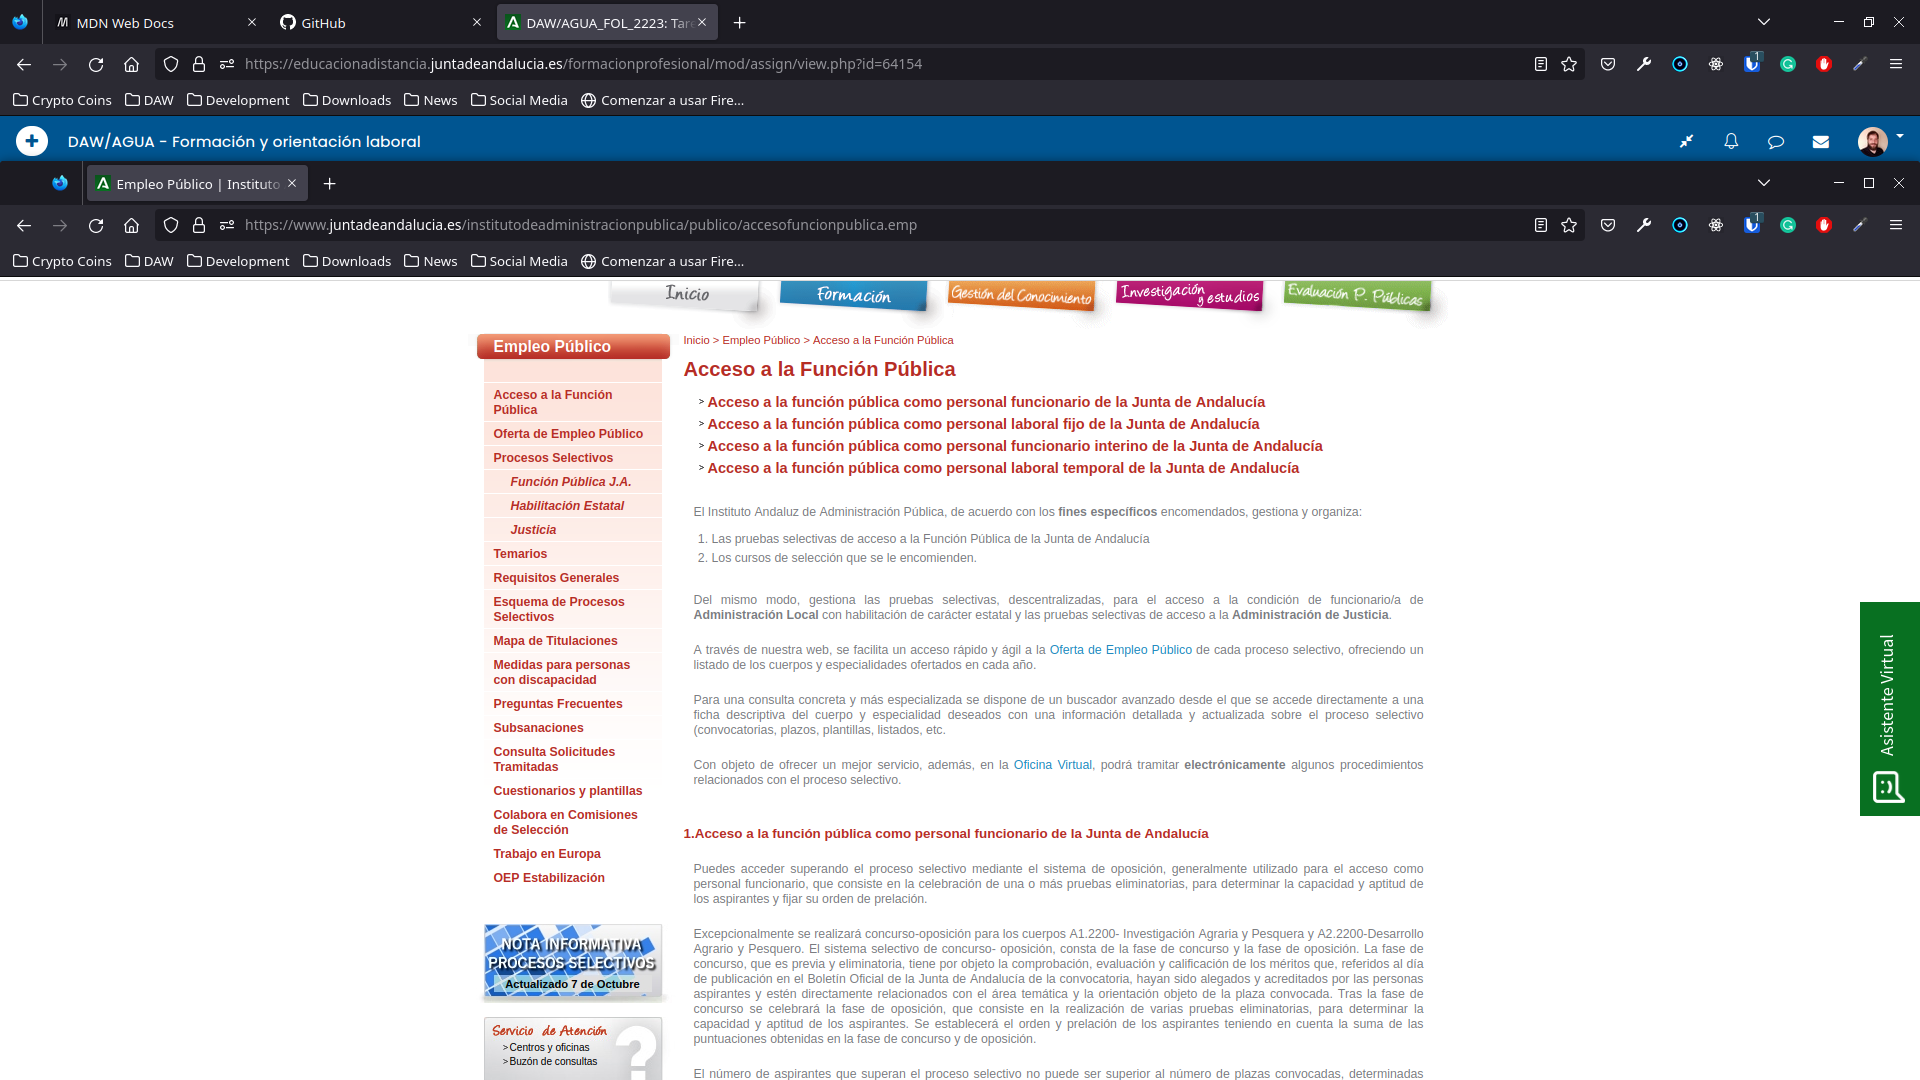
\includegraphics[scale=0.25]{empleo-iaap.png}
        \caption{Sección de Empleo Público del IAAP}
    \end{figure}
\end{enumerate}

\section{Actividad 4}
\subsection{Enunciado}

\begin{enumerate}[label={(\alph*)}]
    \item Realiza una valoración personal reflexionando sobre la importancia de la formación permanente en el sector de la informática y medios a través de los que puedes hacerlo.
    \item Busca una página web/enlace donde aparezca información relacionada con el sector de los estudios que estás cursando ( salidas profesionales, condiciones laborales, oposiciones convocadas,  foros del sector, ofertas de empleo….) Deberás colgarla en el foro y  comentarla. Debes realizar una captura de esta aportación al foro y añadirla a la tarea. La información que subas al foro no podrá haber sido expuesta por otro compañer@ y una sola aportación para que sea igualmente asequible para tod@s.
\end{enumerate}

\subsection{Solución}

\begin{enumerate}[label={(\alph*)}]
    \item En el sector de la informática en general, y más concretamente en el desarrollo de software, la formación continua es imprescindible. Esto se debe a que es un sector muy dinámico donde continuamente están apareciendo nuevas tecnologías, herramientas, paradigmas, etc... Así, es vital para mantener el puesto de trabajo u optar a mejores posiciones la formación continua y la actualización de los conocimientos.

    Los medios de los que nos podemos ayudar para esta formación continua son muy variados. A continuación se muestra una lista con diferentes medios:
    \begin{itemize}
        \item \textbf{Cursos de Formación de la Administración Pública}: tenemos una variedad de cursos de formación y especialización ofertados por las diferentes administraciones públicas. Aquí podemos incluir, por ejemplo, los Cursos de Formación para el Empleo, Formación Ocupacional, Cursos de Especialización, etc... El problema con estos cursos es que el sector del desarrollo de software evoluciona con demasiada rapidez, y los contenidos suelen quedarse desactualizados rápidamente.

        \item \textbf{Plataformas Online de Formación}: tenemos una gran variedad de plataformas online para seguir formándonos. Suelen ofrecer cursos de herramientas o lenguajes específicos, así como de paradigmas concretos. Una de las ventajas es que en muchos casos, estos cursos no solo están bastante actualizados, sino que además están pensados para dedicarles pocas horas a la semana y poder compaginarlos con el empleo. Algunas de las plataformas mas conocidas son: \textbf{Udemy}, \textbf{Coursera}, \textbf{freeCodecamp}, \textbf{eDx}, etc... Además, muchos de estos cursos los imparten algunas de las universidades más punteras del mundo.

        \item \textbf{Documentación Técnica}: este medio es uno de los más usados, y consiste en recurrir a la documentación de los propios creadores de las herramientas o lenguajes. En muchas ocasiones, también ofrecen tutoriales y cursos de diferentes niveles (básico, medio, avanzado). Suele ser la documentación más fiable a la hora de adquirir conocimientos sobre nuevas herramientas y lenguajes, aunque también es la más técnica, por lo que hay que acostumbrarse a usar este tipo de documentación y no requiere más esfuerzo por parte de los profesionales noveles.
    \end{itemize}

    \item En este punto se muestra la captura con el mensaje enviado al foro de la unidad.

        \begin{figure}[ht]
        \centering
        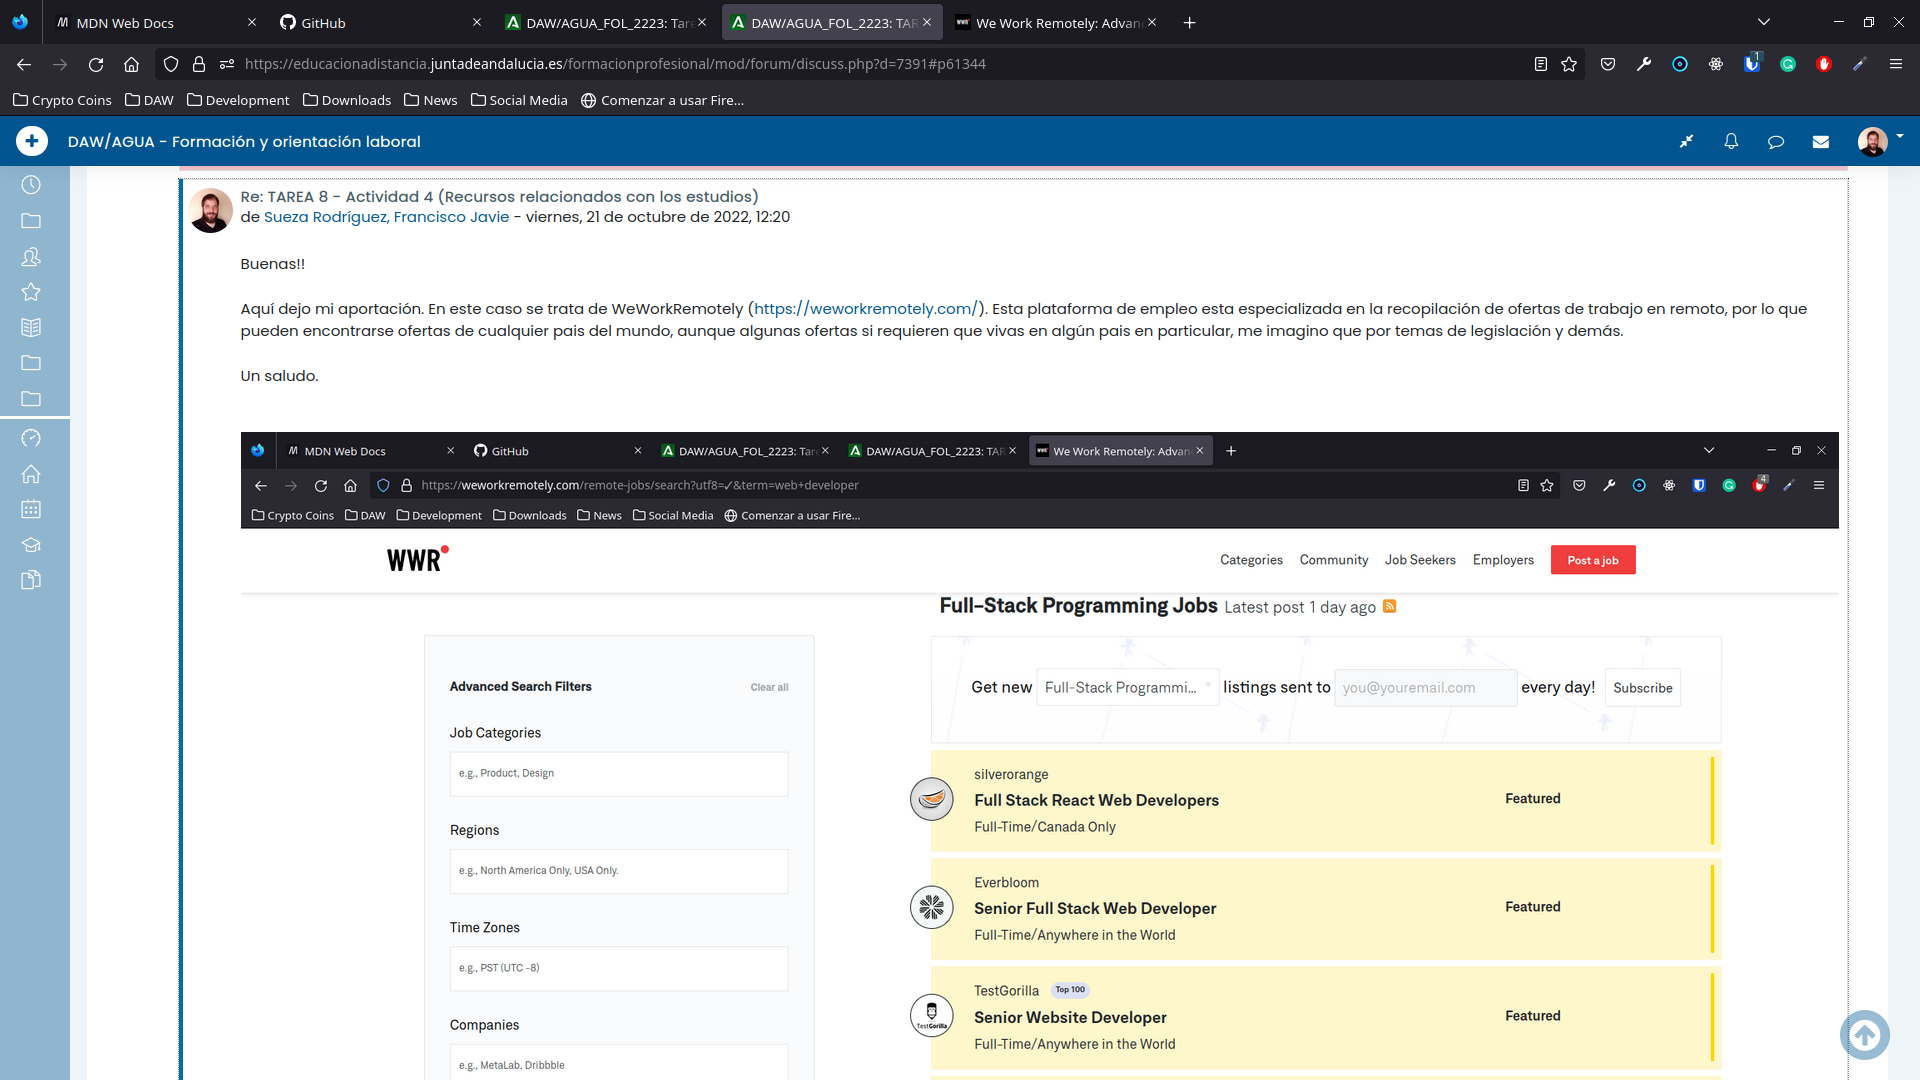
\includegraphics[scale=0.28]{post-foro.png}
        \caption{Captura de mensaje en el foro}
    \end{figure}
\end{enumerate}

\section{Actividad 5}

\subsection{Enunciado}
Tomando de referencia las fases de toma de decisiones del contenido del tema, justifica la elección de estos estudios.

\subsection{Solución}
La elección que tome sobre realizar estos estudios ha sido bien pensada y estudiada. En la siguiente lista, muestro la correspondencia con las fases de toma de decisiones tras la que llegue a esta conclusión:

\begin{enumerate}
    \item \textbf{Reconocimiento}: hace unos años decidí empezar a estudiar informática para sacarme una titulación, ya que aunque ha sido mi hobbie desde joven nunca había ejercido como tal. Entré en la Universidad de Granada para realizar los estudios de Grado en Ingeniería Informática, pero en ese momento también tenía un trabajo en la hostelería que no me permitió dedicarle todo el tiempo que requiere la carrera, por lo que acabé abandonándola. Aún así, yo seguía empeñado en trabajar como programador web.

    \item \textbf{Enumeración de alternativas}: llegados a este punto, tenía dos alternativas:
    \begin{itemize}
        \item \textbf{El Autoempleo}: intentar trabajar como autónomo o montar una empresa.
        \item \textbf{Obtener un título}: si quería encontrar trabajo en alguna empresa como asalariado, tenía que seguir formándome, ya que sin título iba a ser muy complicado encontrar un puestos de trabajo.
    \end{itemize}

    \item \textbf{Análisis de alternativas}: cada una de las dos alternativas tienen sus ventajas e inconvenientes, a saber:
    \begin{itemize}
       \item \textbf{Autoempleo}: está opción tiene la \textbf{ventaja} de que podría facilitarme la inserción en el sector más rápidamente, una mayor parte de los beneficios o poder ponerme yo mismo mis horarios, pero también tiene muchos \textbf{inconvenientes}, requiere de unas competencias y conocimientos en otros ámbitos, como marketing o gestión de empresas que yo en ese momento no tenía (todavía tampoco). Además esta el tema de la gestión, pagos, IVA, búsqueda de clientes, etc...

       En el \textbf{aspecto técnico} también habría algunos \textbf{problemas}, ya que al tener que encargarme desde 0 de todo el proceso de desarrollo debería tener conocimientos de diseño gráfico, algo de lo que carezco. Por lo que esta opción sería la menos ideal.

       Además, cabe la posibilidad de que no consiga clientes, y al final todo el esfuerzo haya sido en vano.

       \item \textbf{Obtener un título}: el principal \textbf{inconveniente} de esta opción es que requiere más tiempo y no va a facilitarme un empleo inmediatamente, en cambio, la principal \textbf{ventaja} es que me va a abrir muchas puertas, incluso si tengo buen ojo y hago un poco de análisis de las ofertas en mi provincia a la hora de hacer las prácticas puedo acabar ya contratado en esa empresa.

       Hay varias opciones para llevar esto a cabo, aunque un requisito es que la formación tiene que ser a distancia, para poder compaginarlo en el caso de que me salga algún empleo de pocas horas durante el proceso.

       Después de evaluar las diferentes opciones, la mejor opción es la de un \textbf{Ciclo Formativo de Grado Superior} a distancia, ya que es la formación que me va a abrir mas puertas, estando por supuesto, descartada la vuelta a la universidad.
     \end{itemize}

     \item \textbf{Elección}: tras analizar las dos opciones, decidí decantarme por \textbf{obtener un título}. Teniendo en cuenta los requisitos de la formación, como el hecho de que tenga que ser a distancia, me informé sobre los Ciclos Superiores a distancia en Andalucía, llegando a la conclusión de que la mejor opción y la que más se ajustaba a mis necesidades era estudiar el \textbf{Ciclo Superior de Desarrollo de Aplicaciones Web} en la \textbf{Oferta Parcial Diferenciada}, por lo que empecé a recopilar información sobre todo el procedimiento de matrícula, calendario, documentación requerida, etc...

     \item \textbf{Ejecución}: con toda la información ya en mi mano, solicite la plaza en varios institutos que ofertaban el ciclo elegido, con la suerte de que me asignaron módulos en el IES Aguadulce. Tampoco es un proceso que no haya tenido contratiempos hasta el momento, como los problemas con las cartas de pago, o el hecho de que solo me asignaran en primera adjudicación solo 2 módulos, lo que alargaría más la obtención del título, pero han sido contratiempos menores y algunos esperados. Este punto aún está en desarrollo, claro.
\end{enumerate}

\section{Actividad 6}
\subsection{Enunciado}
Enumera diferentes técnicas o canales de búsqueda de empleo de diferentes tipos que has utilizado o utilizarás en un futuro próximo.

\subsection{Solución}
A lo largo de mi vida he usado diferentes técnicas de búsqueda de empleo. Aunque actualmente las que más utilizo es internet, he usado otras.

\begin{itemize}
    \item \textbf{Técnicas de Búsqueda Activa}:
    \begin{enumerate}
        \item \textbf{Red de contactos}: en alguna ocasión he usado mi red de contactos que me han informado sobre puestos concretos, la mayoría en hostelería.
        \item \textbf{Prensa}: uno de los puestos que desempeñe como teleoperador lo conseguí gracias a un anuncio en la prensa, aunque no ha sido el medio que más he utilizado.
    \end{enumerate}
    \item \textbf{Técnica Pasivas}:
    \begin{enumerate}
        \item \textbf{Empresas de Trabajo Temporal}: durante un tiempo también estuve apuntado a un par de ETTs, aunque sin mucho éxito.
        \item \textbf{Internet}: en internet ha sido donde he usado más plataformas especializadas en empleo, especialmente Infojobs y Linkedin.
    \end{enumerate}
\end{itemize}

\section{Actividad 7}

\subsection{Enunciado}

\begin{enumerate}[label={\alph*}]
    \item Haz una valoración sobre las ventajas de montar tu propia empresa.
    \item Haz una valoración sobre los inconvenientes de montar tu propia empresa.
    \item Expón si esta posibilidad de autoemplearte cabe en un futuro, la descartas o ya estás en ello.
\end{enumerate}

\subsection{Solución}

\begin{enumerate}[label={(\alph*)}]
    \item Las principales \textbf{ventajas} que tiene montar una empresa son las siguientes:
    \begin{itemize}
        \item \textbf{Mayor libertad y autonomía} en comparación con el trabajo por cuenta ajena, pudiendo elegir horarios, en que clientes centrarnos, forma de trabajar, etc...
        \item \textbf{Mayor parte de los beneficios}. Si la empresa funciona bien, el porcentaje de los beneficios que nos llevamos es mucho mayor.
        \item La \textbf{satisfacción personal} también es mayor que en el trabajo asalariado, ya que el producto lo hemos creado nosotros mismos desde 0 y ver que funciona y a los clientes le gusta es una fuente de satisfacción personal.
    \end{itemize}
    \item Por otro lado los \textbf{inconvenientes} son varios:
    \begin{itemize}
        \item Necesidad de más \textbf{competencias}, ya que además las propias del puesto de trabajo que estemos desarrollando tenemos que poseer las relacionados con la creación y gestión de empresa, marketing, etc...
        \item La \textbf{administración y gestión} de la empresa corre a nuestro cargo, lo que además de ser complejo nos ocupará bastante tiempo, incluso fuera de nuestro horario establecido.
        \item Además, siempre estará el \textbf{riesgo económico} presente, ya que la creación de una empresa requiere inversión de capital que podemos perder si la idea no funciona.
        \item Hay mayor {incertidumbre} en general, un mes podemos tener menos clientes que otro, ganando menos dinero, o podemos tardar más de la cuenta en realizar un trabajo, lo cual hace que tengamos más incertidumbre y menos estabilidad, por lo menos al principio.
    \end{itemize}
    \item Personalmente nunca he montado una empresa, he hecho algunos trabajos por cuenta ajena, pero han sido muy esporádicos y no conllevan todo los inconvenientes ni beneficios de montar una empresa. En un futuro es una opción que nunca he descartado, pero esta claro que necesitaría trabajar más ciertas competencias que no poseo, como en temas de gestión de empresas, marketing, diseño gráfico, etc... Aunque no sería mi opción predilecta.
\end{enumerate}










% Bibliography

\newpage
\bibliography{citas}
\bibliographystyle{unsrt}

\end{document}